\documentclass[11pt,a4paper]{article}

\usepackage{iftex}
\ifPDFTeX
  \usepackage[utf8]{inputenc}
  \usepackage[T1]{fontenc}
  \usepackage{lmodern}
\else
  \usepackage{fontspec} % XeLaTeX / LuaLaTeX / Tectonic
\fi
\usepackage[margin=2.2cm]{geometry}
\usepackage{amsmath}
\usepackage{graphicx}
\usepackage{booktabs}
\usepackage{float}
\usepackage{algorithm}
\usepackage{algpseudocode}
\usepackage{xcolor}
\usepackage{xurl}
\usepackage{hyperref}

\hypersetup{colorlinks=true, linkcolor=black, urlcolor=blue!60!black}
\setlength{\parindent}{0pt}
\setlength{\parskip}{6pt}

% a list of node indices, wrapped freely
\newcommand{\nodelist}[1]{\par\nopagebreak{\small\ttfamily\raggedright #1\par}}

\title{Lab 2: Greedy regret heuristics}
\author{Aleksander Hański, Kacper Kuźnik}
\date{}

\begin{document}
\maketitle

\textbf{Source code:}\\
\url{https://github.com/aleksanderhanski/evolutionary-computation/tree/main/lab2-greedy-regret-heuristics}

% ---------------------------------------------------------------
\section{Description of the problem}

We are given a set of nodes. Each node has $x$ and $y$ coordinates in a plane and a cost. The goal
is to select exactly 50\% of the nodes (rounded up if the number of nodes is odd) and form a
Hamiltonian cycle through the selected nodes, so that the sum of the total length of the cycle and
the total cost of the selected nodes is minimized.

Distances between nodes are Euclidean distances rounded mathematically to integers. The distance
matrix is computed once, right after reading an instance. The optimization methods only use the
distance matrix and the vector of node costs, never the coordinates.

For a solution given as an ordered list of nodes $(v_0, \dots, v_{k-1})$:
\[
  f(v_0, \dots, v_{k-1}) = \sum_{i=0}^{k-1} D[v_i][v_{(i+1) \bmod k}] + \sum_{i=0}^{k-1} \mathit{cost}[v_i]
\]
Both instances, TSPA and TSPB, have 200 nodes, so every solution contains $k = 100$ nodes.

% ---------------------------------------------------------------
\section{Pseudocode of the implemented algorithms}

Notation: $D$ is the distance matrix, $\mathit{cost}$ the node costs, $n$ the number of nodes,
$k = \lceil n/2 \rceil$. As in Lab~1, ``nearest'' is never the plain distance: the change of the
objective function after an insertion always includes the cost of the inserted node.

\subsection*{Insertion cost}
Both new methods are built on the two insertion heuristics from Lab~1. They differ only in the set
of places where a node $v$ can be inserted and in the cost $\Delta(v, p)$ of inserting it at
place $p$.

\textbf{Nearest neighbor (any position)} -- the path is open while it is being built, the edge
closing the cycle only appears in the final solution. The places are $p = 0, \dots, |P|$:
\[
  \Delta(v, p) =
  \begin{cases}
    D[v][P_0] + \mathit{cost}[v] & p = 0 \text{ (before the first node)}\\
    D[P_{|P|-1}][v] + \mathit{cost}[v] & p = |P| \text{ (after the last node)}\\
    D[a][v] + D[v][b] - D[a][b] + \mathit{cost}[v] & \text{otherwise, } a = P_{p-1},\ b = P_p
  \end{cases}
\]

\textbf{Greedy cycle} -- the solution is a closed cycle all the time, so the places are the
$|P|$ edges $(a, b)$ of the cycle, including the edge (last, first):
\[
  \Delta(v, (a, b)) = D[a][v] + D[v][b] - D[a][b] + \mathit{cost}[v]
\]

\subsection*{Regret and the weighted criterion}
For every node $v$ not in the solution let $\Delta_1(v)$ be its smallest and $\Delta_2(v)$ its
second smallest insertion cost over all places. The 2-regret is
\[
  \mathit{regret}(v) = \Delta_2(v) - \Delta_1(v),
\]
i.e.\ how much we lose if we do not insert $v$ now and its best place gets taken. Both methods
select a node by a score, and the selected node is always inserted at its best place:
\begin{itemize}
  \item \textbf{Greedy 2-regret}: $\mathit{score}(v) = \mathit{regret}(v)$,
  \item \textbf{Weighted sum}: $\mathit{score}(v) = w_r \cdot \mathit{regret}(v) - w_b \cdot \Delta_1(v)$,
        with equal weights $w_r = w_b = 1$ by default.
\end{itemize}
The weighted criterion with $w_r = 0$ is the plain greedy method from Lab~1, and with $w_b = 0$ it is
the pure 2-regret heuristic. Ties in the score are broken by the smaller $\Delta_1$, then by the
lower node index.

\subsection*{Nearest neighbor (any position) with 2-regret}
\begin{algorithm}[H]
\caption{Nearest neighbor (any position) with 2-regret}
\begin{algorithmic}[1]
\Function{NNAnyPositionRegret}{$D, \mathit{cost}, \mathit{start}$}
  \State $P \gets [\mathit{start}]$
  \While{$|P| < k$}
    \ForAll{nodes $v \notin P$}
      \ForAll{positions $p \in 0 \dots |P|$}
        \If{$p = 0$} \Comment{before the first node}
          \State $\Delta(v, p) \gets D[v][P_0] + \mathit{cost}[v]$
        \ElsIf{$p = |P|$} \Comment{after the last node}
          \State $\Delta(v, p) \gets D[P_{|P|-1}][v] + \mathit{cost}[v]$
        \Else \Comment{between $a = P_{p-1}$ and $b = P_p$}
          \State $\Delta(v, p) \gets D[a][v] + D[v][b] - D[a][b] + \mathit{cost}[v]$
        \EndIf
      \EndFor
      \State $\Delta_1(v) \gets$ smallest $\Delta(v, \cdot)$, $p^*(v) \gets$ its position
      \State $\Delta_2(v) \gets$ second smallest $\Delta(v, \cdot)$
      \State $\mathit{score}(v) \gets \Delta_2(v) - \Delta_1(v)$
    \EndFor
    \State $v^* \gets \arg\max_v \mathit{score}(v)$ \Comment{ties: smaller $\Delta_1$, then lower index}
    \State insert $v^*$ into $P$ at position $p^*(v^*)$
  \EndWhile
  \State \Return $P$
\EndFunction
\end{algorithmic}
\end{algorithm}

\subsection*{Nearest neighbor (any position) with weighted sum criterion}
\begin{algorithm}[H]
\caption{Nearest neighbor (any position) with 2-regret + best change}
\begin{algorithmic}[1]
\Function{NNAnyPositionWeighted}{$D, \mathit{cost}, \mathit{start}, w_r = 1, w_b = 1$}
  \State $P \gets [\mathit{start}]$
  \While{$|P| < k$}
    \ForAll{nodes $v \notin P$}
      \ForAll{positions $p \in 0 \dots |P|$}
        \If{$p = 0$} \Comment{before the first node}
          \State $\Delta(v, p) \gets D[v][P_0] + \mathit{cost}[v]$
        \ElsIf{$p = |P|$} \Comment{after the last node}
          \State $\Delta(v, p) \gets D[P_{|P|-1}][v] + \mathit{cost}[v]$
        \Else \Comment{between $a = P_{p-1}$ and $b = P_p$}
          \State $\Delta(v, p) \gets D[a][v] + D[v][b] - D[a][b] + \mathit{cost}[v]$
        \EndIf
      \EndFor
      \State $\Delta_1(v) \gets$ smallest $\Delta(v, \cdot)$, $p^*(v) \gets$ its position
      \State $\Delta_2(v) \gets$ second smallest $\Delta(v, \cdot)$
      \State $\mathit{score}(v) \gets w_r \cdot (\Delta_2(v) - \Delta_1(v)) - w_b \cdot \Delta_1(v)$
    \EndFor
    \State $v^* \gets \arg\max_v \mathit{score}(v)$ \Comment{ties: smaller $\Delta_1$, then lower index}
    \State insert $v^*$ into $P$ at position $p^*(v^*)$
  \EndWhile
  \State \Return $P$
\EndFunction
\end{algorithmic}
\end{algorithm}

\subsection*{Greedy cycle with 2-regret}
\begin{algorithm}[H]
\caption{Greedy cycle with 2-regret}
\begin{algorithmic}[1]
\Function{GreedyCycleRegret}{$D, \mathit{cost}, \mathit{start}$}
  \State $P \gets [\mathit{start}]$
  \While{$|P| < k$}
    \ForAll{nodes $v \notin P$}
      \ForAll{edges $(a, b)$ of the cycle $P$, including (last, first)}
        \State $\Delta(v, (a, b)) \gets D[a][v] + D[v][b] - D[a][b] + \mathit{cost}[v]$
      \EndFor
      \State $\Delta_1(v) \gets$ smallest $\Delta(v, \cdot)$, $p^*(v) \gets$ its edge
      \State $\Delta_2(v) \gets$ second smallest $\Delta(v, \cdot)$ \Comment{$= \Delta_1(v)$ while $|P| = 1$}
      \State $\mathit{score}(v) \gets \Delta_2(v) - \Delta_1(v)$
    \EndFor
    \State $v^* \gets \arg\max_v \mathit{score}(v)$ \Comment{ties: smaller $\Delta_1$, then lower index}
    \State insert $v^*$ into $P$ at edge $p^*(v^*)$
  \EndWhile
  \State \Return $P$
\EndFunction
\end{algorithmic}
\end{algorithm}

\subsection*{Greedy cycle with weighted sum criterion}
\begin{algorithm}[H]
\caption{Greedy cycle with 2-regret + best change}
\begin{algorithmic}[1]
\Function{GreedyCycleWeighted}{$D, \mathit{cost}, \mathit{start}, w_r = 1, w_b = 1$}
  \State $P \gets [\mathit{start}]$
  \While{$|P| < k$}
    \ForAll{nodes $v \notin P$}
      \ForAll{edges $(a, b)$ of the cycle $P$, including (last, first)}
        \State $\Delta(v, (a, b)) \gets D[a][v] + D[v][b] - D[a][b] + \mathit{cost}[v]$
      \EndFor
      \State $\Delta_1(v) \gets$ smallest $\Delta(v, \cdot)$, $p^*(v) \gets$ its edge
      \State $\Delta_2(v) \gets$ second smallest $\Delta(v, \cdot)$ \Comment{$= \Delta_1(v)$ while $|P| = 1$}
      \State $\mathit{score}(v) \gets w_r \cdot (\Delta_2(v) - \Delta_1(v)) - w_b \cdot \Delta_1(v)$
    \EndFor
    \State $v^* \gets \arg\max_v \mathit{score}(v)$ \Comment{ties: smaller $\Delta_1$, then lower index}
    \State insert $v^*$ into $P$ at edge $p^*(v^*)$
  \EndWhile
  \State \Return $P$
\EndFunction
\end{algorithmic}
\end{algorithm}

\subsection*{First step}
In the first step every place gives the same insertion cost: the path $[\mathit{start}]$ has two
places (before and after) with equal cost, and the one-node cycle has a single degenerate edge
$(\mathit{start}, \mathit{start})$. All regrets are therefore 0 and the tie-break picks the node
with the smallest $\Delta_1$, as in Lab~1.

% ---------------------------------------------------------------
\section{Results of the computational experiment}

For each greedy method 200 solutions were generated, one starting from each node. 200 random
solutions were generated with a fixed seed (42). The results of the Lab~1 methods were recomputed
in the same run and are identical to the previous report. Values are min / average / max of the
objective function, the best value in each column is in bold.

\begin{table}[H]
\centering
\begin{tabular}{lrrr}
\toprule
Method & TSPA min & TSPA avg & TSPA max \\
\midrule
Random & 240892 & 262956.1 & 289850 \\
NN (end only) & 84362 & 87476.6 & 90075 \\
NN (any position) & 72328 & 74306.5 & 77022 \\
Greedy cycle & 72590 & 73743.7 & \textbf{75281} \\
\midrule
NN (any position) 2-regret & 110950 & 121360.3 & 135771 \\
NN (any position) weighted & 72419 & 75549.4 & 78504 \\
Greedy cycle 2-regret & 112806 & 120378.8 & 128089 \\
Greedy cycle weighted & \textbf{72011} & \textbf{73353.5} & 75532 \\
\bottomrule
\end{tabular}
\end{table}

\begin{table}[H]
\centering
\begin{tabular}{lrrr}
\toprule
Method & TSPB min & TSPB avg & TSPB max \\
\midrule
Random & 186840 & 206333.8 & 227175 \\
NN (end only) & 56007 & 59397.3 & 63166 \\
NN (any position) & 52915 & 59476.2 & 66164 \\
Greedy cycle & 55655 & 59650.8 & 63734 \\
\midrule
NN (any position) 2-regret & 68761 & 73649.8 & 79756 \\
NN (any position) weighted & \textbf{50485} & \textbf{55698.9} & \textbf{61406} \\
Greedy cycle 2-regret & 68150 & 72484.8 & 77274 \\
Greedy cycle weighted & 52731 & 57863.3 & 63370 \\
\bottomrule
\end{tabular}
\end{table}

\subsection*{Other weights}
We also ran the weighted criterion with other weights $(w_r, w_b)$, 200 solutions each.
$(1, 0)$ is the pure 2-regret and $(0, 1)$ the plain greedy method; the latter differs from the
Lab~1 numbers by less than 0.1\% because ties are broken in a different order.
Average objective, best value per row in bold:

\begin{table}[H]
\centering
\begin{tabular}{lrrrrr}
\toprule
Method & $(1, 0)$ & $(2, 1)$ & $(1, 1)$ & $(1, 2)$ & $(0, 1)$ \\
\midrule
TSPA NN (any position) & 121360.3 & 76408.1 & 75549.4 & 75279.7 & \textbf{74347.0} \\
TSPA Greedy cycle      & 120378.8 & 74277.2 & 73353.5 & \textbf{73189.0} & 73793.4 \\
TSPB NN (any position) & 73649.8 & \textbf{54710.1} & 55698.9 & 56150.8 & 59475.5 \\
TSPB Greedy cycle      & 72484.8 & 59659.1 & 57863.3 & \textbf{55714.3} & 59649.9 \\
\bottomrule
\end{tabular}
\end{table}

% ---------------------------------------------------------------
\section{Visualization of the best solutions}

Each panel shows the best solution of one method. Selected nodes are filled, and both their size
and color show the node cost (bigger and darker means more expensive). Nodes that are not selected
are drawn as hollow grey circles, with size still showing their cost. Plots of the Lab~1 methods are
in the previous report.

\subsection*{TSPA}
\begin{figure}[H]
  \centering
  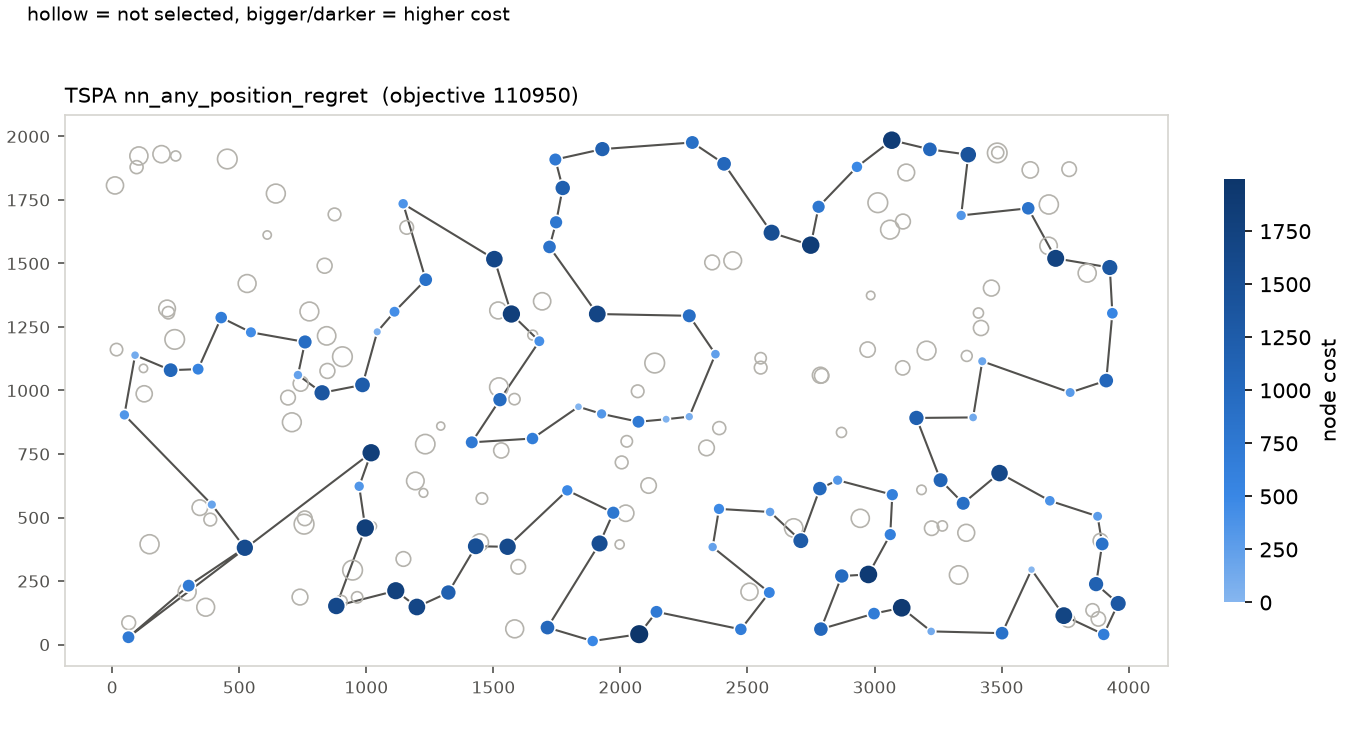
\includegraphics[width=0.85\textwidth]{plots/TSPA_nn_any_position_regret.png}
  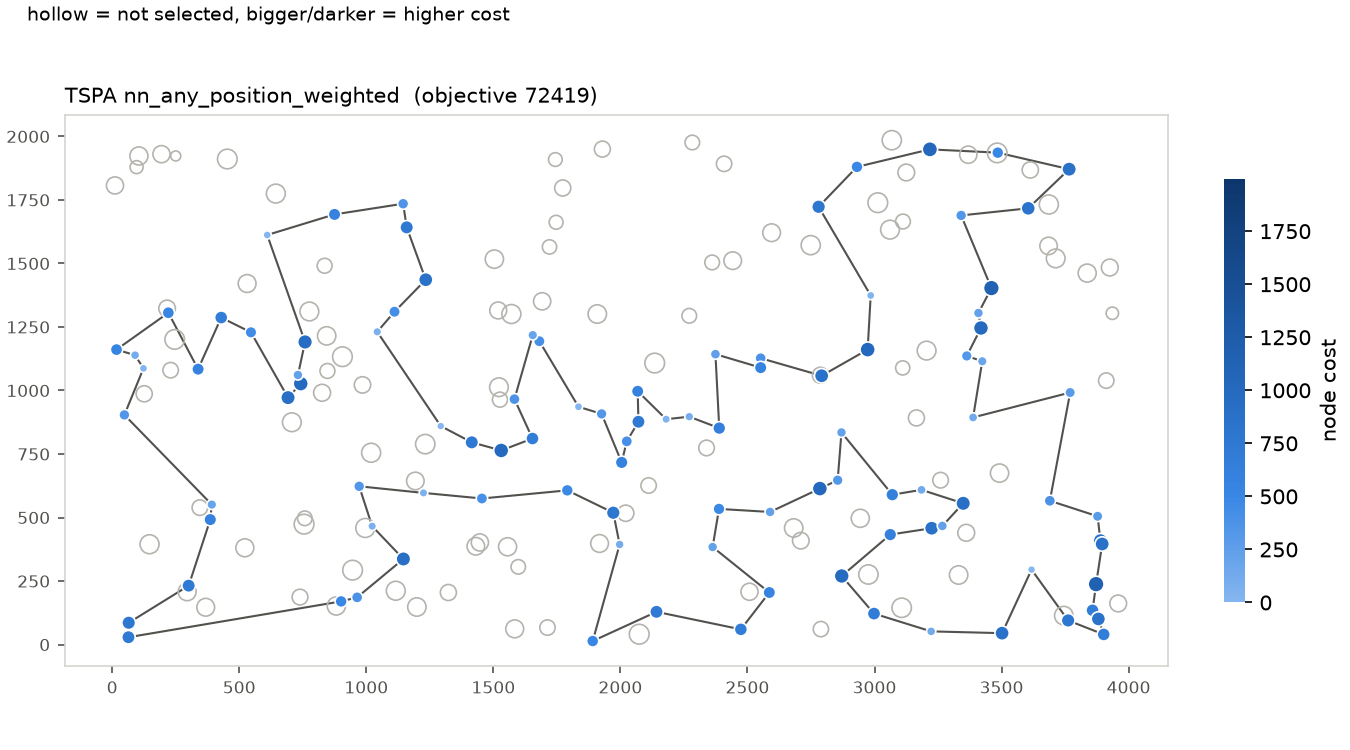
\includegraphics[width=0.85\textwidth]{plots/TSPA_nn_any_position_weighted.png}
\end{figure}
\begin{figure}[H]
  \centering
  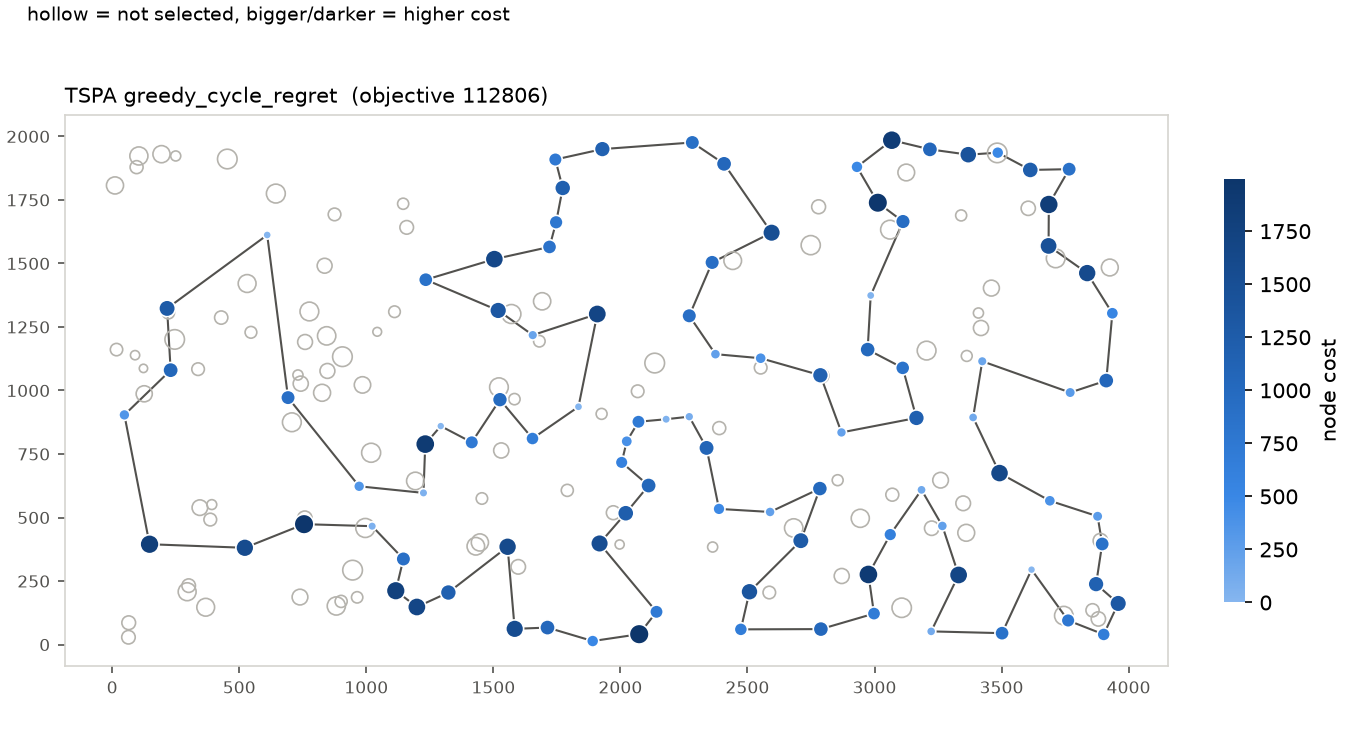
\includegraphics[width=0.85\textwidth]{plots/TSPA_greedy_cycle_regret.png}
  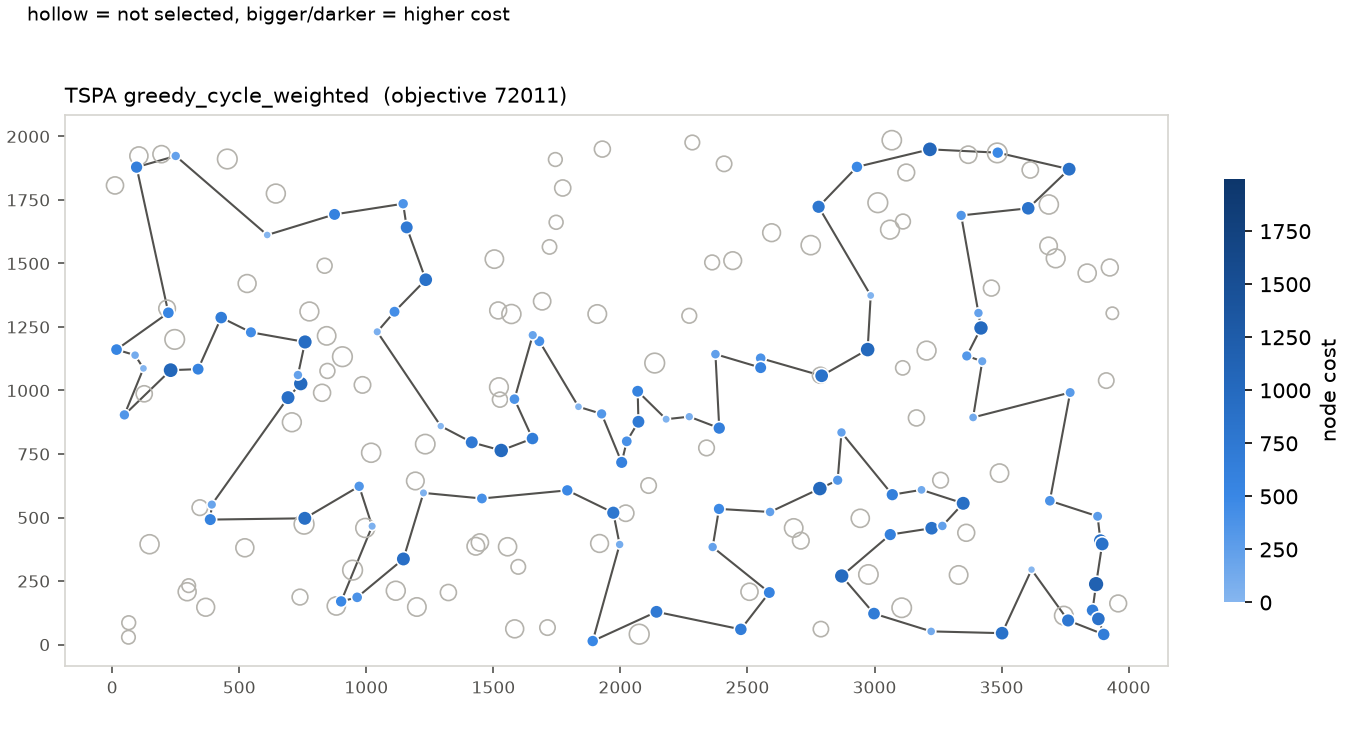
\includegraphics[width=0.85\textwidth]{plots/TSPA_greedy_cycle_weighted.png}
\end{figure}

\subsection*{TSPB}
\begin{figure}[H]
  \centering
  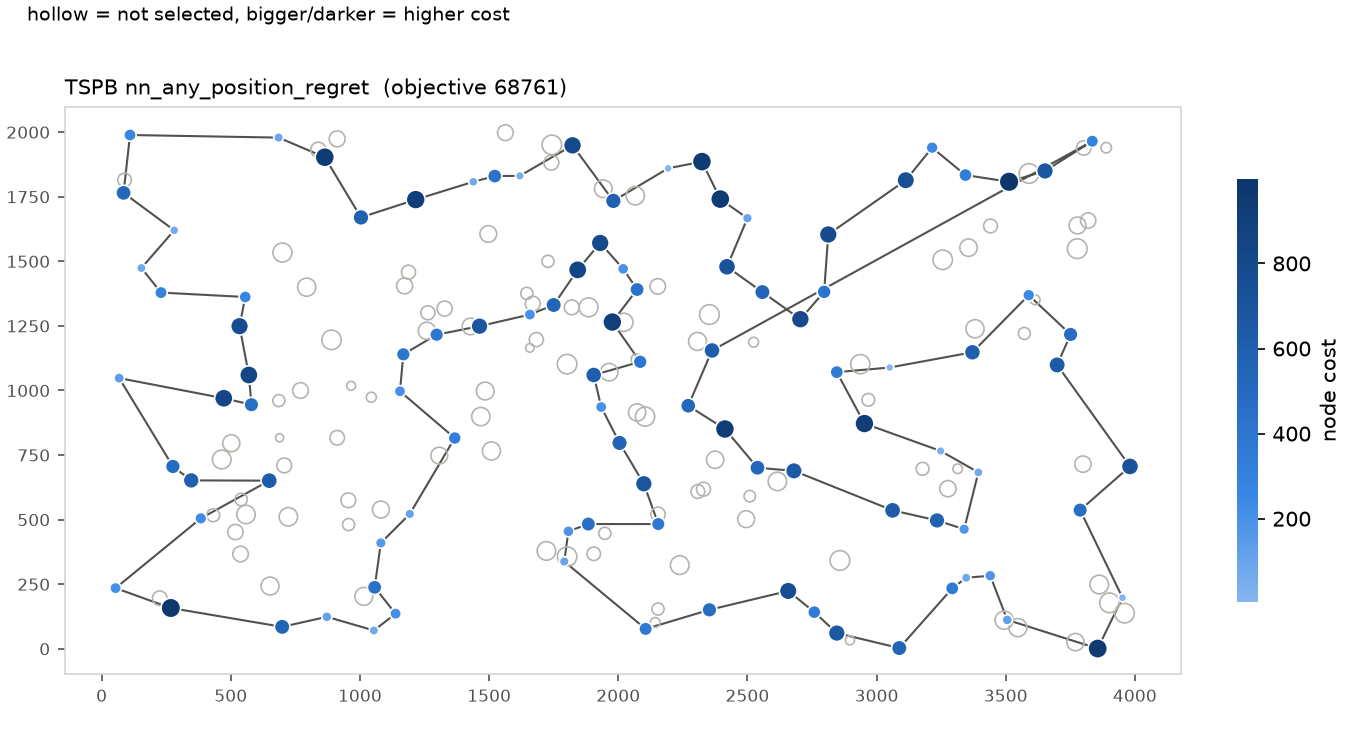
\includegraphics[width=0.85\textwidth]{plots/TSPB_nn_any_position_regret.png}
  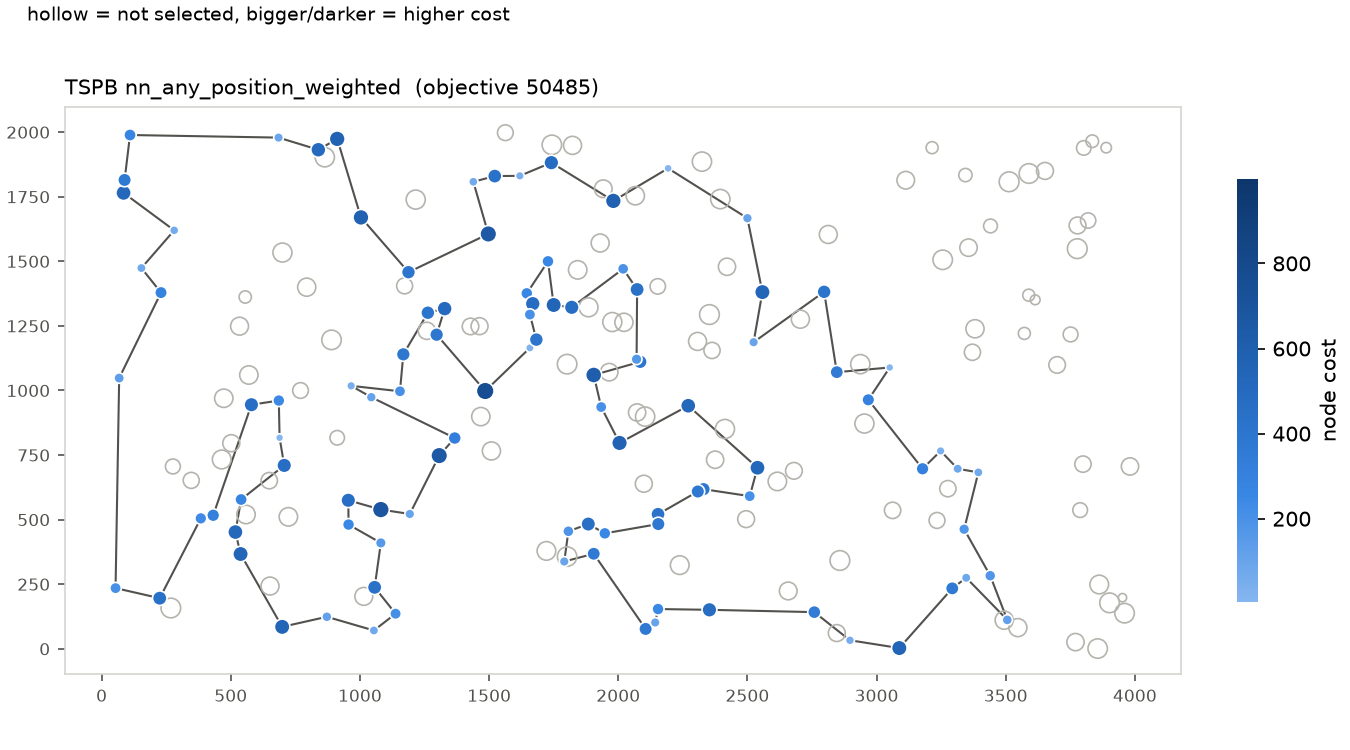
\includegraphics[width=0.85\textwidth]{plots/TSPB_nn_any_position_weighted.png}
\end{figure}
\begin{figure}[H]
  \centering
  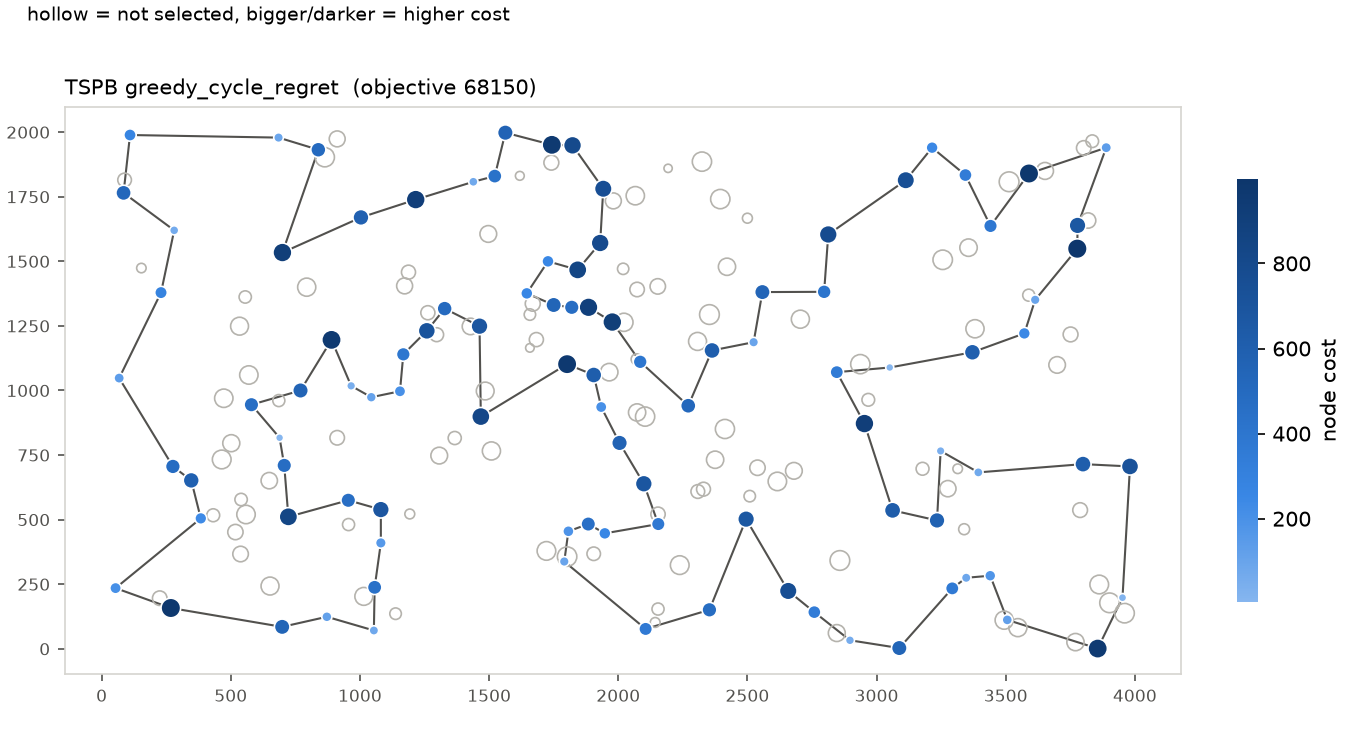
\includegraphics[width=0.85\textwidth]{plots/TSPB_greedy_cycle_regret.png}
  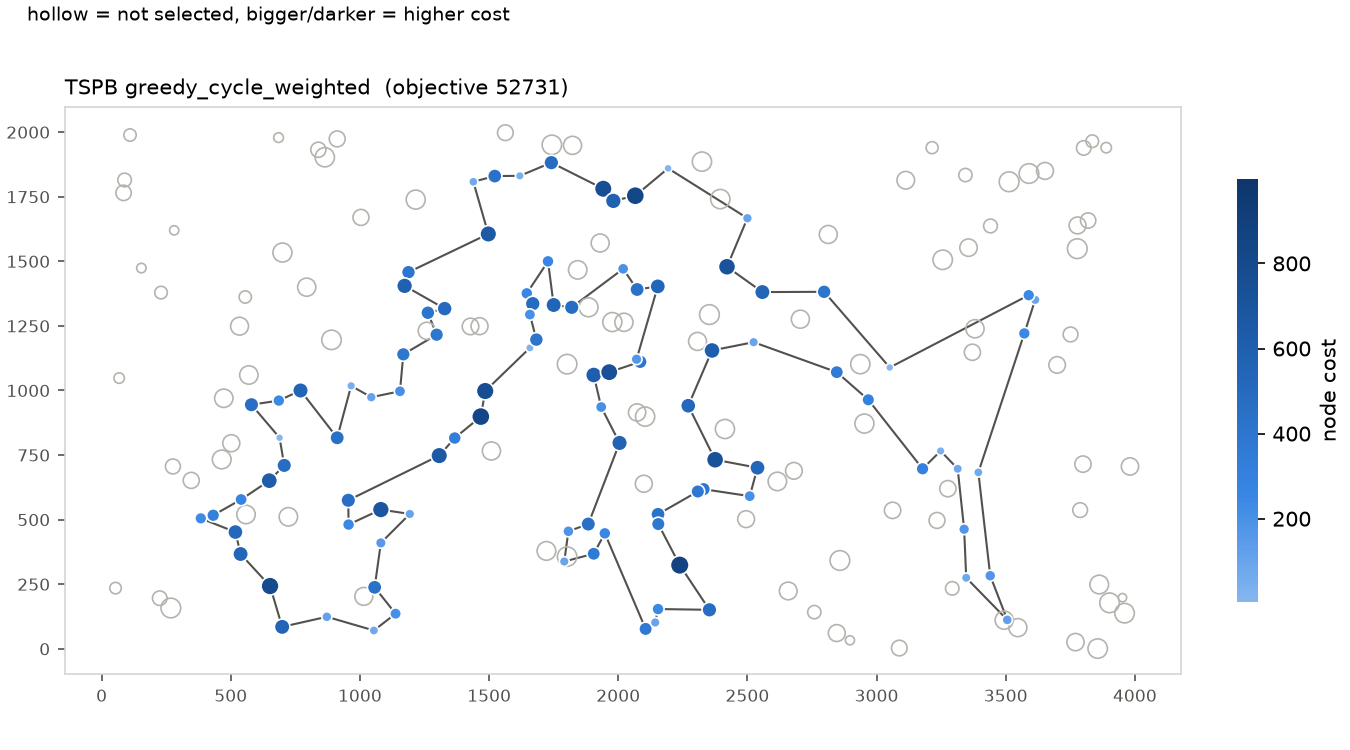
\includegraphics[width=0.85\textwidth]{plots/TSPB_greedy_cycle_weighted.png}
\end{figure}

% ---------------------------------------------------------------
\section{Best solutions}

Lists of node indices, starting from 0, in the order they are visited. The cycle closes from the
last node back to the first. Best solutions of the Lab~1 methods are unchanged and listed in the
previous report.

\subsection*{TSPA}

\textbf{NN (any position) 2-regret} (objective 110950)
\nodelist{104, 69, 120, 97, 168, 149, 11, 49, 108, 152, 100, 123, 148, 162, 132, 76, 4, 157, 18, 173, 16, 156, 28, 185, 67, 144, 179, 177, 36, 33, 143, 190, 139, 112, 5, 115, 175, 39, 154, 34, 109, 186, 136, 197, 163, 19, 178, 101, 155, 21, 147, 37, 47, 50, 93, 81, 43, 113, 117, 130, 159, 170, 75, 26, 78, 122, 107, 64, 57, 105, 182, 111, 138, 165, 151, 150, 176, 72, 65, 134, 84, 58, 158, 192, 181, 118, 114, 25, 121, 73, 45, 70, 96, 10, 183, 166, 32, 40, 30, 23}

\textbf{NN (any position) weighted} (objective 72419)
\nodelist{171, 2, 189, 187, 30, 141, 87, 45, 73, 135, 114, 181, 192, 158, 58, 84, 134, 72, 176, 174, 150, 106, 113, 89, 42, 151, 138, 182, 57, 64, 107, 88, 78, 193, 153, 75, 170, 146, 159, 130, 47, 93, 50, 3, 169, 1, 59, 178, 101, 55, 29, 163, 136, 186, 164, 142, 8, 9, 54, 33, 131, 36, 177, 52, 179, 53, 140, 144, 67, 16, 51, 35, 185, 102, 28, 180, 132, 76, 4, 71, 157, 91, 80, 100, 123, 83, 160, 152, 108, 49, 60, 116, 149, 63, 168, 97, 127, 69, 129, 104}

\textbf{Greedy cycle 2-regret} (objective 112806)
\nodelist{166, 183, 10, 70, 22, 25, 114, 118, 181, 121, 61, 41, 140, 53, 179, 177, 36, 99, 84, 134, 72, 65, 20, 192, 111, 182, 165, 151, 106, 89, 124, 57, 64, 107, 88, 78, 26, 75, 170, 159, 130, 117, 93, 50, 47, 37, 147, 6, 46, 86, 55, 17, 29, 19, 163, 197, 136, 195, 184, 164, 142, 85, 81, 174, 194, 9, 33, 143, 62, 34, 154, 39, 175, 115, 5, 112, 139, 18, 4, 196, 51, 190, 67, 185, 156, 28, 180, 191, 141, 30, 160, 80, 82, 11, 168, 188, 120, 125, 187, 189}

\textbf{Greedy cycle weighted} (objective 72011)
\nodelist{60, 116, 149, 63, 168, 11, 49, 108, 152, 100, 123, 83, 160, 97, 127, 161, 30, 187, 171, 2, 189, 141, 87, 45, 73, 135, 114, 181, 192, 158, 58, 84, 134, 72, 176, 174, 150, 106, 113, 89, 42, 151, 138, 182, 57, 64, 107, 88, 78, 193, 153, 75, 170, 146, 159, 130, 47, 93, 50, 3, 169, 1, 178, 101, 55, 29, 163, 136, 186, 164, 142, 8, 9, 54, 33, 131, 36, 177, 52, 179, 53, 140, 144, 67, 16, 51, 35, 185, 102, 28, 180, 132, 76, 4, 71, 157, 91, 80, 48, 31}

\subsection*{TSPB}

\textbf{NN (any position) 2-regret} (objective 68761)
\nodelist{94, 169, 199, 70, 190, 194, 77, 104, 144, 185, 79, 57, 83, 44, 89, 156, 164, 96, 198, 121, 195, 50, 7, 116, 37, 13, 149, 28, 145, 158, 138, 55, 177, 53, 65, 178, 103, 180, 132, 1, 108, 62, 175, 134, 45, 157, 60, 40, 64, 47, 38, 21, 168, 172, 8, 92, 166, 72, 46, 109, 3, 122, 151, 98, 25, 181, 73, 59, 85, 82, 88, 163, 99, 39, 17, 74, 20, 14, 2, 23, 110, 118, 131, 143, 148, 196, 78, 54, 162, 106, 127, 90, 153, 182, 150, 84, 66, 35, 27, 135}

\textbf{NN (any position) weighted} (objective 50485)
\nodelist{65, 145, 28, 149, 13, 146, 37, 116, 147, 42, 50, 130, 63, 121, 198, 96, 48, 156, 89, 57, 185, 76, 104, 162, 54, 192, 80, 127, 129, 90, 153, 14, 2, 20, 74, 17, 171, 99, 88, 179, 87, 82, 51, 85, 59, 73, 167, 181, 152, 34, 24, 67, 66, 27, 98, 151, 122, 3, 184, 46, 72, 117, 8, 120, 133, 136, 172, 160, 69, 124, 21, 183, 30, 38, 47, 154, 140, 64, 33, 40, 141, 155, 71, 60, 157, 45, 134, 175, 62, 36, 197, 6, 115, 170, 125, 177, 29, 132, 174, 1}

\textbf{Greedy cycle 2-regret} (objective 68150)
\nodelist{167, 181, 25, 98, 151, 122, 128, 4, 168, 183, 176, 38, 47, 140, 154, 161, 26, 177, 170, 115, 113, 155, 141, 60, 157, 134, 175, 62, 108, 1, 132, 103, 178, 65, 145, 149, 13, 37, 116, 147, 123, 50, 195, 121, 198, 58, 16, 164, 43, 166, 92, 120, 133, 8, 117, 95, 109, 3, 27, 135, 76, 185, 104, 77, 194, 190, 70, 187, 165, 105, 139, 193, 114, 10, 78, 54, 162, 106, 150, 182, 127, 90, 56, 131, 110, 23, 2, 14, 20, 74, 17, 171, 99, 163, 31, 88, 82, 85, 59, 73}

\textbf{Greedy cycle weighted} (objective 52731)
\nodelist{36, 197, 132, 29, 6, 180, 115, 170, 177, 125, 26, 97, 154, 140, 47, 38, 21, 30, 183, 191, 130, 63, 121, 198, 96, 48, 43, 156, 32, 89, 57, 79, 185, 104, 54, 196, 114, 10, 90, 14, 2, 20, 153, 129, 127, 80, 192, 162, 76, 135, 27, 11, 66, 67, 24, 34, 152, 181, 126, 88, 179, 87, 82, 167, 51, 85, 59, 73, 98, 151, 122, 173, 3, 184, 86, 46, 72, 117, 8, 120, 133, 136, 172, 160, 69, 124, 4, 64, 33, 155, 71, 141, 40, 60, 157, 45, 134, 175, 62, 91}

% ---------------------------------------------------------------
\section{Solution checker}

All sixteen best solutions (eight per instance, including the Lab~1 methods) were checked with the
provided solution checker (\texttt{Solution checker.xlsx}), and every objective value matches. Our
code additionally checks every generated solution for the number of nodes and for repeated nodes.

\begin{table}[H]
\centering
\begin{tabular}{llrrc}
\toprule
Instance & Method & Our objective & Checker objective & Match \\
\midrule
TSPA & Random & 240892 & 240892 & yes \\
TSPA & NN (end only) & 84362 & 84362 & yes \\
TSPA & NN (any position) & 72328 & 72328 & yes \\
TSPA & Greedy cycle & 72590 & 72590 & yes \\
TSPA & NN (any position) 2-regret & 110950 & 110950 & yes \\
TSPA & NN (any position) weighted & 72419 & 72419 & yes \\
TSPA & Greedy cycle 2-regret & 112806 & 112806 & yes \\
TSPA & Greedy cycle weighted & 72011 & 72011 & yes \\
\midrule
TSPB & Random & 186840 & 186840 & yes \\
TSPB & NN (end only) & 56007 & 56007 & yes \\
TSPB & NN (any position) & 52915 & 52915 & yes \\
TSPB & Greedy cycle & 55655 & 55655 & yes \\
TSPB & NN (any position) 2-regret & 68761 & 68761 & yes \\
TSPB & NN (any position) weighted & 50485 & 50485 & yes \\
TSPB & Greedy cycle 2-regret & 68150 & 68150 & yes \\
TSPB & Greedy cycle weighted & 52731 & 52731 & yes \\
\bottomrule
\end{tabular}
\end{table}

% ---------------------------------------------------------------
\section{Conclusions}

\begin{itemize}
  \item The pure 2-regret heuristic is clearly worse than the plain greedy methods: about 120\,000
        on average on TSPA (vs.\ 73\,744 for greedy cycle) and about 73\,000 on TSPB (vs.\ 59\,651).
        The node cost is the same at every place, so it cancels out in
        $\Delta_2(v) - \Delta_1(v)$ and the regret does not see it at all. The tour lengths are
        similar (21\,429 for the best greedy cycle 2-regret solution on TSPA vs.\ 21\,570 for
        greedy cycle), but the selected nodes cost 91\,377 instead of 51\,020. The plots show this:
        the regret solutions contain many large, dark nodes.
  \item The weighted criterion (2-regret + best change, equal weights) fixes this and gives the best
        results of all methods so far. On TSPA greedy cycle weighted has the best minimum (72\,011)
        and average (73\,353.5, 0.5\% below greedy cycle). On TSPB the gain is larger: NN (any
        position) weighted has the best minimum, average and maximum (50\,485 / 55\,698.9 /
        61\,406), its average is 6.4\% below NN (any position), and greedy cycle weighted improves
        the greedy cycle average by 3.0\%.
  \item The regret term mainly shortens the tour: the best greedy cycle weighted solution on TSPB has
        length 16\,365 vs.\ 19\,634 for greedy cycle, with almost the same node cost (36\,366 vs.\
        36\,021). Nodes whose good insertion places are about to disappear are inserted early, so
        the method leaves fewer long detours and crossings.
  \item The weights matter, and no single pair is the best everywhere. Putting more weight on the
        best change, $(1, 2)$, gave the best greedy cycle averages on both instances (73\,189.0 and
        55\,714.3), while NN (any position) on TSPB was best with more weight on regret, $(2, 1)$.
        On TSPA, NN (any position) did not gain from the regret term on average. Equal weights are a
        reasonable default: never the worst choice, and always far better than the pure 2-regret.
  \item The regret methods cost almost nothing extra: they need the same insertion costs as the
        greedy methods, plus the second smallest value per node. Our simple Python implementation
        takes about 70\,ms per solution.
\end{itemize}

\end{document}
